\documentclass{beamer}

\title{TMAT3004}
\subtitle{Bruk av maskinsyn for deteksjon av ulike fiskearter}

\author{Hans Alan Whitburn Haugen}

% Hvordan lage en god visuell presentasjon
%  Bruk en enkel mal (gjerne NTNU-mal)
%  Unngå «information overload»
%  Stikkord eller korte setninger
% Test presentasjonen på forhånd 

\begin{document}
	\frame {

	% Få erfaring med å presentere innenfor en gitt tidsramme og takle spørsmål
	% Få tilbakemelding på prosjektet fra medstudenter og veileder
	% Få tilbakemelding på innhold og form fra hovedveileder
	% Få innblikk i andres oppgaver, bidra med kommentarer og få ideer til egen presentasjon

% Min oppgave handler om maskinsyn. Oppgaven er gjort i samarbeid med Nofima.

		\titlepage
	}
	\frame {
		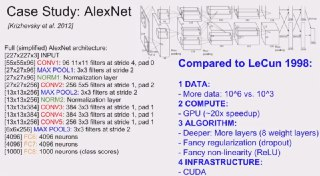
\includegraphics[scale=0.2]{../report/figures/alexnet}
	}
	\frame {

% Hva skal vi si?

		% Hva går arbeidet vårt ut på?
		\frametitle{Undersøkelse}
		\framesubtitle{Fôrsprengt fisk}
		
%\section*{Sammendrag}

%Lengre oppgaver, som bachelor- og masteroppgaver, skal ha et sammendrag. Det er viktig at sammendraget er informativt, siden det skal kunne leses av lesere som ikke er eksperter på området.

%Sammendraget skal være kort, helst ikke over én A4-side, og skal gi et overblikk over hovedinnholdet. Du skal fortelle leseren:

%hva du har undersøkt

%Fôrsprengt fisk har blitt vanlig i Lyngen kommune i Troms. “Pellets-fisk” ble vanlig etter at de begynte med oppdrett i fjorden. Fisken er full av fôr og stinker. Den er unaturlig og tjukk.

%``Pellets-fisk'' er villfisk som har spist oppdrettsfôr som inneholder medisin. Denne fisken blir omsatt. Et eksempel er når lakselusmiddelet emamectin ble gitt til oppdrettfisk i tre uker i 2017 i denne fjorden i Lyngen. Oppdrettsfisken var i karantene i denne perioden, og blir ansett som giftig. I samme periode leverte fiskere villfisk fra denne fjorden til et mottak i Troms. Den var full av pellets. Det sto ut av munnen på både sei og torsk.

%Det er et ønske å kartlegge omfanget av problemet, og fiskere vil ha svar på om pellets-fisken kan være farlig. Det er et ønske å kartlegge hvor mange villfisk som trekker til oppdrettsanlegg, og under hvilke forhold. Sjømatdivisjonen og Akvadivisjonen ved Nofima har en strategisk internsatsing å samle kunnskap om sameksistens mellom ulike marine næringer og interesser, deriblant hvordan man kan unngå konflikter mellom ulike interesser.

%Dette prosjektet har gått ut på å lage programvare for Nofima som kan skape en oversikt over mengden fisk av typen torsk og sei som beiter rundt oppdrettsanlegg, og som viser fordelingen av fiskeartene til forskjellige tider på døgnet.

%hvordan du gjorde det

%Maskinlæring er når datamaskiner lærer fra data. I 2012 vant AlexNet Stanford University sin årlige ImageNet bildeklassifiseringskonkurranse. Teamet til Alex anvendte deep learning og det har revolusjonert maskinsyn og kunstig intelligens. Flere modeller har blitt laget siden AlexNet, og bildeklassefisering, objektdeteksjon og segmentering har blitt mye mer nøyaktig nå som de anvender dype kunstige neurale nettverk. Facebook introduserte RetinaNet i 2017, og i 2018 kom YOLOv3. Det er disse teknologiene som har blitt anvendt til å lage en modell som kan kjenne igjen torsk og sei med ...(resultater) .

%hva du fant ut

%Prosjektet viser at maskinsyn kan anvendes til å løse oppgaver innenfor akvakultur. Teknologien som presenteres i dette dokumentet kan anvendes til å finne omfanget av torsk og sei som beiter rundt oppdrettsanlegg, og kan muligens anvendes til å detektere rømninger fra merder samt utvikles videre til å detektere lakselus på fisk i merdene.

		% Fiskere og oppdrettsnæringen er i konflikt. Kystfiskere hevder villfisken får i seg så mye laksefôr at fiskeplassene blir ødelagt. ``Litt overraskende utspill'' svarer oppdrettsbransjen. Fisker Tor Inge Larsen i Brønnøysund sa til NRK i 2018 at han fortviler over det han mener er dårligere kvalitet hos fisken han fanger. Han sa han kan knapt huske sist han fikk en sei om bord i båten uten at den hadde pellets fra lakseoppdrett i magen. Han hevder fiskerne har blitt frastjålet fiskeområder på høylys dag, og mener fiskefeltene nært Brønnøysund på Sør-Helgeland i Nordland har fått betydelig lavere kvalitet på grunn av oppdrettsanleggene

		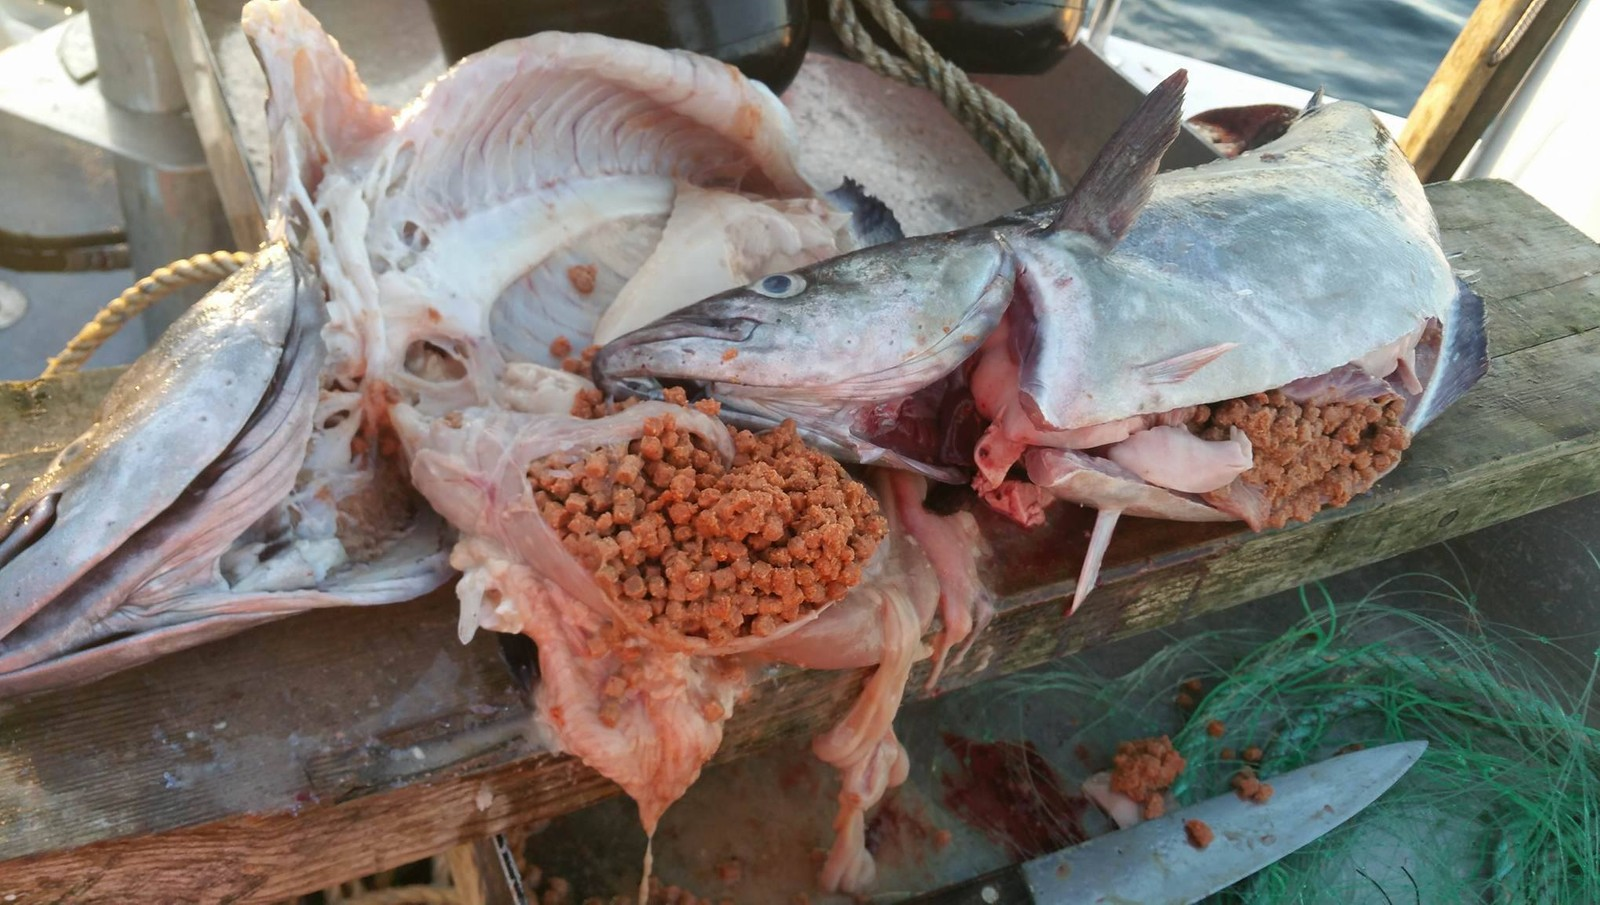
\includegraphics[scale=0.2]{../report/figures/oppdrettfor}

		%\[\frac{-b \pm \sqrt{b^2 - c}}{2a}\]
	}
%	\frame {
%
%		\frametitle{Hvorfor?}
%		\framesubtitle{Fôrsprengt fisk}
%		
%		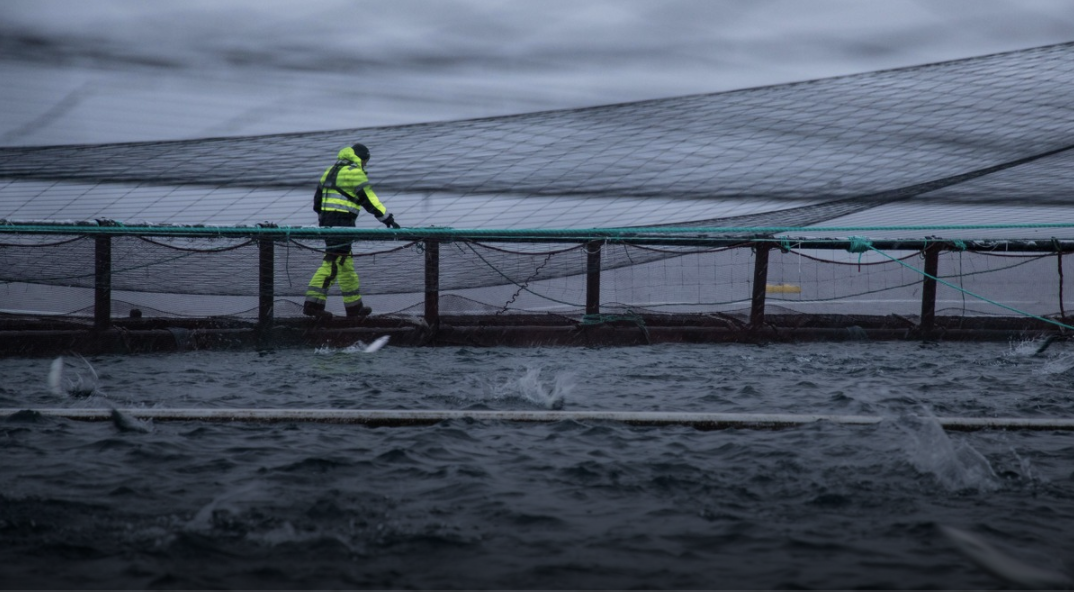
\includegraphics[scale=0.6]{../report/figures/oppdrett}
%
%		%\[\frac{-b \pm \sqrt{b^2 - c}}{2a}\]
%	}
	\frame{
		% Mål – nytteverdi (for samarbeidspartner, for samfunnet, for oss)
		\frametitle{Demo}
		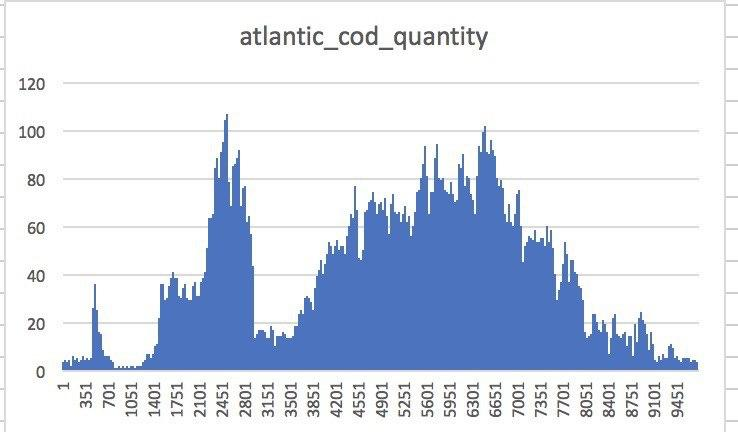
\includegraphics[scale=0.4]{graph}
	}
	\frame{
		\frametitle{Videre utvikling}
		%\framesubtitle{Nofima}
		\begin{itemize}
			\item Seidata
			\item Segmentering

		%	\item Maskinsyn
		%	\item YOLOv3
		%	\item RetinaNet
		\end{itemize}
	}

	\frame{
	    % Be om forslag/kommentarer?
	    \frametitle{Forslag eller kommentarer?}
	    %This is a paragraph.
	}
\end{document}
